\documentclass[12pt,halfline,a4paper,nonumbib]{ouparticle}

%\usepackage[authoryear]{natbib}

\usepackage[backend=biber,
            style=authoryear,
            %citestyle=authoryear,
            maxcitenames=1,
            sorting=nyt]{biblatex}
\addbibresource{references.bib}

%% My definitions
\usepackage{xcolor}
\newcommand{\toshi}{\textcolor{blue}}
\newcommand{\disp}{\displaystyle}

\usepackage{algorithm}
\usepackage{algorithmicx}
\usepackage{algpseudocode}


\begin{document}

\title{Validation of stock assessment models. Is it me or my model talking? }

\author{%
\name{Laurence T. Kell}
\address{ Centre for Environmental Policy, Imperial College London, Weeks Building, 16-18 Princes Gardens, London\\ SW7 1NE, UK}
\email{laurie@seaplusplus.co.uk}
\and
\name{Rishi Sharma}
\address{Food and Agricultural Organization, Fishery and Aquaculture Policy and Resources Division, Rome, Lazio,\\
00153, Italy}
\email{rishi.sharma@fao.org}
\and
\name{Toshihide Kitakado}
\address{Department of Marine Biosciences, Tokyo University of Marine Science and Technology, 4-5-7 Konan, Minato, Tokyo \\108-8477, Japan}
\email{e-mail address}
\and
\name{Henning Winker}
\address{Joint Research Centre (JRC), European Commission, TP 051, Via Enrico Fermi 2749, 21027 Ispra, VA, \\Italy.}
\email{e-mail address}
\and
\name{Iago Mosqueira}
\address{Wageningen Marine Research, Haringkade 1, 1976CP IJmuiden, \\The Netherlands.}
\email{iago.mosqueira@wur.nl}
\and
\name{Massimiliano Cardinale}
\address{Swedish University of Agricultural Sciences, Department of Aquatic Resources, Institute of Marine Research, Lysekil,\\ Sweden}
\email{massimiliano.cardinale@slu.se}
\and
\name{Dan}
\address{x}
\email{xx}}

\abstract{

The adoption of the Precautionary Approach requires a consideration of uncertainty, which is commonly addressed by the use of alternative stock assessment model structures or by fixing key parameters. Evaluating  model fits in such cases is difficult, however, using traditional goodness-of-fit diagnostics based on likelihoods and model residuals. While retrospective analysis based on model outputs can not be used for validation as this requires a reference set of observations. Furthermore these methods merely tells us how well we describe the past, but little about how well we can predict the future under alternative management actions. Therefore, we use hindcasting to estimate prediction skill for three alternative model structures using the Indian Ocean yellowfin tuna assessment as a case study. 

The approach can be used to develop robust advice, either by estimating current stock status for an ensemble of models or by weighting Operating Models when conducting Management Strategy Evaluation. For example backcasting is used in risk modelling to evaluate the performance of alternative strategies. This requires simulating past conditions which is simple with the hindcast. Conducting Management Strategy Evaluation as part of a backcast allows the impact of feedback that affect historical catches and stock status to be evaluated. Hindcasting also provides insights that may not be available when models and strategies are tested on simulated data.
}

\date{\today}

\keywords{cross-validation, diagnostics, hindcast, retrospective analysis, stock assessment, validation}

\maketitle



\begin{itemize}
%\item consequences for YFT and validation and data
\item link to metrics
\item Sidney quote
\end{itemize}

\section{Introduction}

There are various definitions of stock assessment \parencite[e.g.][]{hilborn2003state,cadrin2014stock}. Our preference is for "The description of the characteristics of a 'stock' so that its biological reaction to being exploited can be rationally predicted and the predictions tested" (Holt pers comm.). Our reasoning is this explicitly recognises that the main aim of a stock assessment is to provide the basis for the long-term sustainable management of fisheries resources. Stock assessment, therefore, requires making and validating probabilistic estimates of stock status and forecasts of the consequences of management actions.

Stock assessment is a critical element of fisheries management, and diagnostic tests are essential for determining the robustness of model estimates \parencite{carvalho2020cookbook}. Particularly since the adoption of the Precautionary Approach to fisheries management \parencite[PA,][]{garcia1996precautionary} requires a formal consideration of uncertainty, which is often addressed by the use of alternative modelling frameworks, assumptions and datasets. It can be challenging, therefore, to use diagnostics based on likelihoods and model residuals to compare models. An alternative is to use hindcasting to evaluate prediction skill \parencite{huschke1959glossary} by comparing model estimates to known values, i.e. by withholding recent data and predicting for the period omitted. Hindcasting can either be model based by comparing model estimates, or model-free by generating pseudo observations. The pseudo data are then compared to a reference set of observations \parencite{jin2008current, weigel2008can, balmaseda1995decadal}. Prediction skill can help to validate models by identify model misspecification, data conflicts and where models need to be extended. As a worked example, we compare three model families used for the assessment of Indian Ocean yellowfin tuna stock, namely a full integrated statistical model (SS), an age-structured production model (ASPM), and a Bayesian state-space biomass dynamic model (JABBA). 

Model validation is essential in many fields, e.g. in energy and climate modelling \parencite{kell2019optimising}, as this increases confidence in the outputs of a model and leads to an increase in trust amongst the public, stake and asset-holders and policymakers \parencite[][]{saltelli2020five}. Therefore, after a model structure has is agreed and parameters estimated, it is crucial to validate the model. Validation assesses whether it is plausible that a system identical to the model generated the data \parencite{thygesen2017validation}. The ambition of validation is not to prove that a model is correct, but to check that the model cannot be falsified with the available data. A different question from asking is the model fit for a given purpose, which depends on the intended use of the model. For example to evaluate whether an assessment model can help achieve maximum sustainable yield (MSY)  requires conducting Management Strategy Evaluation \parencite[MSE,][]{punt2007developing}; see \cite{sharma2020trfmo} for a review of current practice in the tuna Regional Fisheries Management Organisations (tRFMOs).    

Model validation serves a purpose complementary to model selection and hypothesis testing. Model selection searches for the most suitable model within a specified family, hypothesis testing examines how to reduce the model structure, and model validation examines if the model family should be modified or extended. For models to be valid, they must satisfy four prerequisites \parencite{hodges1992you}. Namely, the situation modelled must: i) be observable and measurable; ii) be possible to collect sufficient data informative about it; iii) Exhibit constancy of structure in time; and iv) exhibit constancy across variations in conditions not specified in the model

The first two prerequisites should be straight forward; however, many stock assessments (e.g. for highly migratory stocks such as yellowfin tuna fished in areas beyond national jurisdiction), rely on fishery-dependent data rather than direct scientific observations. The use of fishery-dependent data is a concern since \cite{harley2001catch} found strong evidence that commercial catch per unit effort (CPUE) is likely to remain high while abundance declines.  Prerequisite (iii) ensures that the model has prediction skill for the same conditions under which the validation tests were conducted, and prerequisite (iv) ensures that the model will still be valid under conditions that differ from those in the validation tests.

A standard tool in stock assessment to check the stability of model estimates is retrospective analysis \parencite{hurtado2014looking}, which involves sequentially removing data from the most recent years, refitting the model and comparing the time series of spawning stock biomass (SSB) and fishing mortality. Stability of historical estimates, however, can be achieved at the expense of the accuracy and precision of future forecasts, for example by shrinking terminal estimates towards recent historical values. We, therefore, extend the retrospective analysis by projecting forward for the reported catch over the years removed. The use of model-based quantities, however, is not sufficient to fulfil prerequisite i). We, therefore, conduct model-free hindcasts to estimate prediction skill. This is the main objective of the paper, as current literature (e.g. Methot and Wetzel 2013, Prager 1991) primarily focuses on the past, and how well models do fitting these data. Historical performance, however, is no indicator of how well a model may perform in the future, and the hindcasting tool developed here demonstrates how to test alternative models for prediction skill.  


\section{Material and Methods}
Indices of abundance are a key contributor to the overall likelihood when fitting stock assessment models to data \parencite{whitten2013accounting}, and the sum of squared errors (SSE) between observed and predicted indices in log-space is the measure of fitness. When comparing models, however, the SSE is problematic because complex models tend to have many parameters to allow flexibility when fitting, which may result in a low SSE due to overfitting. Therefore, information criteria, such as AIC, have been developed to aid in model selection. AIC is only a relative measure of the appropriateness of models, however, and additional diagnostic tests are required for model validation. This is of particular importance for stock assessment models where only a single historical data set   exists, and the system can not be observed directly. 

The objective of this study therefore is to devlop a procedure to validate and compare different families of models based on past events. To do this we extend retrospective analysis to conduct model-based and model-free hindcasts, by adding the additional step of projecting over the truncated years. Comparing model outputs with observations allows prediction skill to be estimated \parencite{kell2016xval}, defined as any measure of the accuracy of a forecasted value compared to the actual (i.e. observed) value that is not known by the model \parencite{glickman2000glossary}. 

\subsection{Materials}

For our example we use the stock assessment of yellowfin tuna (\textit{Thunnus albacares}) conducted by the Indian Ocean Tuna Commission \parencite{IOTWPTT21}. Yellowfin tuna supports one of the largest tuna fisheries in the Indian Ocean, with catches currently exceeding 400,000t. They are harvested by a variety of gears, from small-scale artisanal fisheries, to large gillnetters, and industrial longliners and purse seiners \parencite{fiorellato2019tt}.

The main assessment is conducted using Stock Synthesis \parencite[SS,][]{methot2013stock}, although other methods are also employed. SS implements an age and spatially structured model that reflects the complex population and fishery dynamics of the stock. Model development has focused on spatial structure to account for the differences in regional exploitation patterns, incorporating seasonal movement dynamics, resolving data conflicts, and exploring non-stationary in selectivity and catchability \parencite{urtizberea2018yft}. The data used includes time series of total catch and four CPUE indices based on the long-line fisheries, spatially stratified in four regions (figure \ref{fig:map})
 
The most recent assessment established a base case as a reference model for diagnostics along with scenarios to capture a range of uncertainties \parencite{fu2018yft}. The assessment indicates that the stock  has declined substantially since 2012, and spawning stock biomass in 2017 is now estimated to be close to the historical lowest level. The stock is estimated to be overfished, and so the IOTC has implemented a rebuilding plan to reduce overall fishing pressure.  

The base case is spatially disaggregated into two tropical regions that encompass the main year-round fisheries and two austral, subtropical regions where the long-line fisheries occur more seasonally \parencite{langley2015yft}, with reciprocal movement assumed to occur between adjacent regions. The SS assessment is based on a quarterly time step to approximate the continuous recruitment and rapid growth seen in the stock. Twenty-five fisheries were defined based on fishing gear, region, time period, fishing mode and vessel type. Most fisheries were modelled allowing flexibility in selectivity (e.g. cubic spline or double normal), whereas long-line selectivity was constrained to be fully selective for the older ages. The population comprised 28 quarterly age-classes with an assumed unexploited equilibrium initial state in each region. 

Recruitment occurs in the two equatorial regions with temporal deviates in the regional distribution and was assumed to follow a Beverton and Holt stock recruitment relationship (with a steepness of 0.8 and recruitment standard deviation of 0.6).  Growth was parameterised using age-specific deviates on the $k$ growth parameter to mimic the non-von Bertalanffy growth of juvenile and the near linear growth of adults. Natural mortality is variable with age, with the relative trend in age-specific natural mortality based on the values applied in the Pacific Ocean \parencite{maunder2012review}. 

%[Maunder, M.N., Aires-da-Silva, A. 2012. A review and evaluation of natural mortality for the assessment and management of yellowfin tuna in the eastern Pacific Ocean. External review of IATTC yellowfin tuna assessment. La Jolla, California. 15-19 October 2012. Document YFT-01-07.]

The data used for fitting are catch and length composition data, long-line CPUE indices, tagging recaptures, and environmental data. The length composition was weighted such that they were sufficient to provide reasonable estimates of fishery selectivity and recruitment trends but not directly influence the trends in stock abundance. Regional environmental indices (current and sea temperature) allows seasonal and temporal variations to be incorporated in the estimation of fish movement. 

The CPUE indices represent the primary source of information on abundance and is based on a composite long-line index from the main distant water fleets %\parencite{hoyle2018yft}. 
Indices in each region were standardised using generalised linear models that accounted for differences in targeting practices and catchability amongst fleets, based on gear configurations and species composition. The reason for this is because tuna long-line fishing strategies have changed over time %\parencite{hampton2005}. 
In the assessment, the CPUE indices across regions were linked by a common catchability coefficient, thus improving the ability of the model to estimate the distribution of biomass by region. %\parencite{langley2015yft, fu2018yft}.

Tag release/recovery data collected from the main phase of the Indian Ocean large-scale tuna tagging programme %[Hallier 2008] 
were integrated into the model to inform estimates of fishing mortality, abundance, and movement. 

%[Hallier 2008. STATUS OF THE INDIAN OCEAN TUNA TAGGING PROGRAMME - RTTP-IO. IOTC-2008-WPTDA-10]

\subsection{Assessment Methods}

There has been a recent trend in stock assessment toward the use of integrated analysis that combines several sources of data into a single model by a joint likelihood for the observed data \parencite[e.g.][]{doubleday1976least,fournier1982general,maunder2013review}. Datasets include records of catches and landings, indices of abundance based on catch per unit (CPUE) or from research surveys, and length and age compositions based on samples. An example of commonly used integrated assessment method is SS3 that can be configured in multiple ways, allowing for a range of scenarios to be developed to reflect uncertainty.

For example \cite{maunder2015contemporary} proposed a deterministic implementation of an age-structured production model (ASPM) as a diagnostic of process dynamics. Selectivity in ASPM is parameterised based on the selectivity estimated by a "full" SS model. The model is then fitted to the abundance indices, assuming a deterministic spawning recruitment relationship, and without the size composition data contributing to the likelihood function. This enables an evaluation of whether the observed catches alone can explain trends in the index of abundance. If the ASPM is able to fit the indices of abundance well then a production function is likely to exist (i.e. the dynamics are driven by density dependent processes), and the indices provide information about absolute abundance. If  the fit is poor, then the catch data alone cannot explain the trends in the indices. This can have several causes, namely (i) stock dynamics are recruitment-driven, (ii) the stock has not yet declined to the point at which catch is a major factor influencing abundance; (iii) the indices of relative abundance are not proportional to abundance;  (iv) the model is incorrectly specified; or (v) the data are incorrect

The ASPM has been shown \parencite{carvalho2017can} to be the best method for detecting misspecification of the key systems-modeled processes that control the shape of the production function. This is a problem since many of the required parameters in integrated assessments are difficult to estimate \parencite[e.g.][]{lee2011m,lee2012steepness} and have to be fixed or priors used. 

An alternative to an integrated assessment is to use a biomass dynamic model, based on an explicit production function, that requires the estimation and fixing of fewer parameters. An example is JABBA, an open source package that presents a unifying, flexible framework for biomass dynamic modelling, runs quickly, and generates reproducible stock status estimates \parencite{winker2018jabba}.The model uses a Pella Tomlinson production function that allows the shape of the production function to be varied, and alternative assumptions about productivity, stock status and reference points to be evaluated. 

The base case SS assessment conducted by the Indian Ocean Tuna Commission (IOTC) for Yellowfin Tuna, was reconfigured as an ASPM and as a biomass dynamic assessment. In the later case in order to mimic the dynamics of the base case assessment, the production function parameters were tuned to the base case Stock synthesis assessment. 

\subsection{Hindcast}

Retrospective analysis \parencite{hurtado2014looking} is commonly used to evaluate the stability of stock assessment estimates from alternative models. Observations are sequentially removed from the terminal year, the model is then refitted to the truncated series and the difference between between estimates from the full and truncated time-series compared using the relative error (RE, a measure of bias). 

Hindcasting like traditional retrospective analysis involves fitting a model using a tailcutting procedure, where data are deleted sequentially for $n$ years, i.e. from the last year $T$ through to $T−n$, the additional step in the hindcast is that then the data from year 1 to $T - n - 1$ are used to make predictions of what will happen in years $T - n$ to $T$.

Since assessment cycles are typically for three years  with advice \parencite{fricker2013three} we projected the truncated estimates for 3 years. We chose 3 years as that is essentially the time-step between assessments in most tuna Regional Fisheries Management Organisations.

\begin{algorithm}[!ht]
\begin{algorithmic}[1]
\State Fit model up to and including terminal year $T$
\For{$t$ = $T - 3$ to n} 
\State fit model to data up to time $t$ \For {$i$ = $t$ to $t + 3$} 
\State Estimate $\hat{y_i}$
\EndFor
\EndFor
\caption{Hindcast}
\label{Hindcast}
\end{algorithmic}
\end{algorithm}

When conducting the hindcast it is assumed that modelled variables are observable, processes exhibit constancy of structure in time, including those not specified in the model, and that collection of accurate and sufficient data is possible \parencite{hodges1992you}.

\subsubsection{Prediction Skill}


The use of model based quantities means that bias can not actually be quantified. For example a reduction in both relative error (a measure of bias) and mean squared error (a measure of variance) can be achieved by shrinking terminal estimates towards recent historical values, at the expense of prediction skill. The absence of retrospective patterns in model based quantities, therefore, while reassuring is not sufficient for model validation, and model-free validation using prediction residuals should be used as well.

Inspection of residuals is a common way to determine a model’s goodness-of-fit \parencite{cox1968general}, since  non-random patterns in the residuals may indicate model misspecification, serial correlation in sampling/observation error, or heteroscedasticity. When inspecting residuals, however, there is a danger of hypothesis fishing/testing?, i.e. [I read the sentence below a few times but could not make sense of it probably need revising?] choosing a scenario retrospectively retrospect, while if multiple true hypotheses are tested it is likely that some of them will be rejected. Therefore it is valuable to reserve part of the data to test for validation, so that a pattern’s significance is not tested on the same data set which suggested the pattern \parencite{thygesen2017validation}. For this reason we conduct a model-free hindcast to estimate prediction skill.

\subsubsection{Metrics}

For the evaluation of model-based quantities, we use Mohn's rho ($\rho_M$ \toshi{$\rho_{Mr}$?}, equation \ref{eqn:mohn}) and a modified version ($\rho_{Mr}$ \toshi{$\rho_{p}$?}, equation \ref{eqn:mohn2}). \toshi{IF my understanding above on $\rho_{p}$ is correct, this is also for assessing prediction skill but "model based". I think we can highlight here difference in model-based and model-free in addition to model validation with/without prediction.}

We used the mean absolute scaled error (MASE, equation \ref{eqn:mase}) to evaluate prediction skill. The best statistical measure to use depends, however, on the objectives of the analysis and using more than one measure can be helpful in providing insight into the nature of observation and process error structures \parencite{kell2016xval}. Therefore we also use root mean squared error ($E^{\prime 2}$, equation \ref{eqn:rmse}), correlation ($\rho$) and the standard deviation ($\sigma$). 

$E^\prime$ is a commonly used metric, as the square root of a variance it can also be interpreted as the standard deviation of the unexplained variance,  lower values indicate better fits. $E^\prime$ is sensitive to outliers, however,and favours forecasts that avoid large deviations from the mean and cannot be used to compare across series. The correlation ($\rho$) in contrast is unaffected by the amplitude of the variations, insensitive to biases and errors in variance, and can be used to compare across series. $E^{\prime 2}$ and $\rho$ are related by the cosine rule i.e.

 \begin{equation} 
 E^{\prime 2} = \sigma_o^2 + \sigma_f^2 - 2\sigma_o\sigma_f\rho
 \end{equation}

Where the reference set ($o$) are the observations not included in the retrospective assessment and the values ($f$) are their estimates. 
 
This means that $E^\prime$, $\rho$ and $\sigma_f$ can be summarised simultaneously in a single diagram\parencite{taylor2001summarizing} providing a concise statistical summary of how well patterns match each other and are therefore especially useful for evaluating multiple aspects or in gauging the relative skill of different models \parencite{griggs2002climate}.

\section{Results}

The retrospective analysis and the three step ahead predictions are shown in figure \ref{fig:retro}. These show the estimates of SSB and F relative to their maximum sustainable yield ($MSY$) reference points  $B_{MSY}$ and $F_{MSY}$. The retrospective analysis shows that SS base case and JABBA assessments are biased, and bias increases for the projection.  For SS, there is over estimation of SSB and underestimation of F, while JABBA shows a strong negative retrospective pattern in F and negative bias in biomass. Although for JABBA  $F:F_{MSY} \le 1$ stock biomass declines below $B_{MSY}$.

The analysis is summarised in Tables \ref{tab:retro-rho} for Monh's $\rho$. Mohn's $\rho$ has to be in the range $[-0.15,0.2]$ for an assessment to be accepted then (Hurtado-Ferro et al., 2014). All the assessments apart from the base case estimates of F pass the Mohn's $\rho$ test for the retrospective analysis. When the 3 year projection is considered, however, all models other than the ASPM fail. Relative error is harder to interpret. 


The results from the model-free hindcasts are shown in Figures~\ref{fig:hy} and \ref{fig:hy3} for the one and three year ahead predictions respectively. The background colour indicates whether MASE < 1, see Table \ref{tab:mase} for the MASE values. For the base case and JABBA, prediction skill is poor for CPUE indices 2 and 3; the ASPM also performs poorly for Area 2. Prediction skill further deteriorates for the three step ahead projection, particularly for the base case and JABBA; although for ASPM, CPUE indices 1 and 3 still have good prediction skill. Area 1 is the centre of the stock distribution (move this sentence to methods).

The fits are summarised in Figures~\ref{fig:td} in the form of Taylor diagrams. Although for the one year projection most models appear to have prediction skill, for the three year hindcast the base case and JABBA perform poorly. The model and prediction residuals are summarised in Figure \ref{fig:residuals} over a five year horizon, these show that SS is imprecise and biased and that while JABBA is more precise, it is also biased.

From our analysis the following can be discerned with respect to how well each models with respect to the current status quo in evaluating models, i.e. retrospective analysis. We then present the model free evaluating algorithms with hindcast for one and three year ahead projections. 

The ASPM appears not to show patterns in the projections, CPUE index 2 performs poorly across all models. The difference between the base case is that it uses length composition data, while JABBA does not model the different regions. It therefore, appears that the length compositions add noise and that area effects (JABBA) are important. 


\section{Discussion}

This paper aimed to support the definition of stock assessment as the description of the characteristics of a ’stock’ so that its biological reaction to being exploited can be rationally predicted and the predictions tested. There are many aspects of stock dynamics and productivity about which there is little information in stock assessment datasets \parencite[e.g.][]{lee2011m,lee2012steepness, jiao2012modelling,simon2012effects,pepin2015reconsidering,cury2014resolving}. A motivation was, therefore, to ensure that stock assessment advice is robust to uncertainty, hypotheses about different plausible states of nature are represented by alternative model structures, fixed parameters, and weighting of data components \parencite[][]{sharma2020trfmo}. 

Model selection, however, based on traditional methods like Akaike’s Information Criteria  \parencite[AIC,][]{akaike1998information} is only suitable for comparing frameworks based on the same input data. Meanwhile, there is a danger, with diagnostics based on the inspection of residuals, of "hypothesis fishing" or "p-hacking" \parencite{wasserstein2016asa,head2015extent}, i.e. finding a pretext for excluding an index or adding extra parameters \parencite[e.g.][]{schirripa2017hypothesis} to improve the fit. If multiple true hypotheses are tested, some of them will likely be rejected falsely. Thus, it is valuable to reserve part of the data for model-free validation, so that a pattern’s significance is not tested on the same data set that suggested the pattern \citep{arlot2010survey}. Therefore, we propose the use of hindcasting with cross-validation to evaluate prediction skill and show how to extend retrospective analysis to do this.

As an example, three structurally different model families were used to assess the yellowfin tuna stock in the Indian Ocean. It was found that the model with the best prediction skill was ASPM. The poor performance of the integrated assessment model is likely related to large, sampling error in the length composition data, which therefore introduce noise rather than information in the estimated recruitment deviations. The Bayesian state-space biomass dynamic model, by contrast, produced reasonable performance metrics for the core fishing area (Region 1) and the south-western Indian Ocean (Region 3), but could not predict the diverging trends in CPUE for Eastern Indian Ocean Region. It appears that it is important to model both the age structure and spatial dynamics for this stock, while the quality of length samples needs to be improved. This illustrates the value of the approach since in the tRFMOs current practice is to run multiple models to evaluate uncertainty and provide advice on, while the evaluation of the value-of-information, the weighting and extension of models is still a research topic \cite{kell2016quantification}. 

If models are used for forecasting, then they should be validated, which requires that model predictions are compared to observable and measurable properties of the system \parencite{ianelli2016multi}. The accuracy and precision of the predictions depend on the validity of the model, the information in the data, and how far ahead we wish to predict (i.e. the prediction horizon). If a model is not validated then, although it may not be possible to use it for prediction, there are still other uses, which include scenario modelling or to use the model as part of a feedback management system. An example might be conducting MSE to develop harvest strategies that are robust to the impacts of environmental forcing or species interactions. To do this requires Operating Models, however, to be conditioned on assumptions other than those used in stock assessment models. A reason for this is because trends and fluctuations in populations are determined by complex interactions between extrinsic forcing and intrinsic dynamics \parencite{bjoernstad2004trends, botsford2014cohort}. Such low-frequency fluctuations can potentially mimic or cloak critical variation in abundance linked to environmental change, over-exploitation or other types of anthropogenic forcing. As advice frameworks move towards ecosystem-based fisheries management (EBFM), a broader range of processes will need to be considered \parencite{ianelli2016multi}. Which will require a greater number of plausible models to describe the system. Therefore, as well as methods for identifying uncertainties and agreeing on scenarios (Leach et al. 2014)there is a need for methods to weight, reject, and extend models to include alternative hypotheses, and to evaluate the value-of-information associated with different datasets.


\section{Conclusions}

 The use of integrated assessment models has meant that fitting to all available data has become commonplace, as scientists seek to use these models to capture all knowledge about stock size and productivity \parencite{hilborn2003state}. Key questions, as when fitting any model, are (i) is my model valid? and (ii) do I have sufficient data and knowledge to fit it? In other words, is it me or my model talking? This is of particular importance for stock assessment, which generally relies on existing stock assessment packages or model frameworks. Stock assessment is generally different from other situations where a model is built from first principles, and diagnostics are applied at each stage of development. In our experience in stock assessments, when someone asks if it is a "good" assessment, they are more likely to be asking about the catch forecast than the goodness of fit diagnostics. We therefore used hindcasting to estimate prediction skill, which in the case study clearly showed that spatial structure is required, but that the length composition sampling error is too large to estimate year-class dynamics, and thus length composition data should be either omitted from the model or revisited.
 
 
Hindcasting enables objective comparison among models with different structures and datasets, which is challenging to do with conventional diagnostics based on likelihoods and model residuals. The hindcast procedure was based on a commonly used diagnostic, retrospective analysis, but these were then extended by adding a forecast. Retrospective analysis allows the temporal stability of advice to be evaluated using a reference series of model estimates based on the most recent assessment. It is not possible, however, to estimate bias associated with prediction skill in this way by using model-based and thus latent quantities. Instead, model estimates need to be compared to observations for objective model validation. The retrospective hindcast was therefore modified to evaluate prediction skill by cross-validating indices of abundance not used in fitting against pseudo observations, i.e. their model estimates. Helping to identify over-fitting and allows exploration of how models can be improved based on alternative structural assumptions without the risk of ‘hypothesis fishing’. 

The approach can also be used with an ensemble of models to develop robust advice, either for estimates of current stock status or by conducting MSE. For example backtesting is the process of evaluating the relative performance of alternatives strategies by comparing these to historical results, and is used in financial risk modelling to assess the performance of a trading or investment strategy. This requires simulating past conditions which is simple with the hindcast. While conducting MSE as part of the backtest allows the impact of feedback on historical catches and stock status to be evaluated. A problem is that it is possible to find a strategy that would have worked well in the past, but will not work well in the future. Therefore, although a backtest MSE is useful, particularly as it allows stakeholders to see what the consequences would have been if a different strategy had been employed, it is not sufficient to ensure the robustness of a strategy to be applied in the future. Despite this limitation, backtesting provides insights that may not be available when models and strategies are tested on simulated data alone and can be performed before conducting MSE for future years.

Another promising field of applications is to use the hindcast procedure to weight multi-model ensembles using simple skill-based weighting. Here, a prediction skill score can be used to assign more weight on the better performing models as this has been found to improve forecasts \parencite[e.g.][]{casanova2009weighting}. This can be done to weight estimates of current status relative to reference points, or weight operating models. Testing the approach on an actual case study first was informative as it provides the insight necessary to set up a study on synthetic data.


\clearpage
\newpage
\printbibliography

\section{Tables}

\begin{table}[!ht]
\caption{Mohn's ($\rho_{Mr}$) for retrospective analysis.}  
\begin{center}
\label{tab:retro-rho}
\begin{tabular}{|cccc|}
\hline
	\tiny Method	& {\tiny Quantity}  & {\tiny Retrospective} & {\tiny Projection} \\ 
\hline\hline
{\tiny SSB          } & {\tiny SS} 	     & {\tiny    0.04} & {\tiny  0.32}      \\
{\tiny SSB          } & {\tiny ASPM} 	 & {\tiny   -0.03} & {\tiny -0.09}      \\
{\tiny SSB          } & {\tiny JABBA} 	 & {\tiny   -0.09} & {\tiny -0.21}      \\
{\tiny F            } & {\tiny SS} 	     & {\tiny   -0.15} & {\tiny -0.24}      \\
{\tiny F            } & {\tiny ASPM} 	 & {\tiny    0.03} & {\tiny  0.08}      \\
{\tiny Harvest Rate } & {\tiny JABBA} 	 & {\tiny   -0.09} & {\tiny -0.09}      \\
\hline
\end{tabular}
\end{center}
\end{table}

\begin{table}[ht]
\caption{Model-free results}
\centering
\label{tab:mase}
\tiny
\begin{tabular}{|cc|ccc|ccc|ccc|ccc|}
  \hline
 CPUE & Quarter &  & MASE &  &  & RMSE & &  & $\rho$ &  & & $\sigma$ &  \\
      &         & SS & ASPM & JABBA & SS & ASPM & JABBA & SS & ASPM & JABBA & SS & ASPM & JABBA \\
\hline\hline
  1 & 1 & 1.04 & 0.56 & 0.98 & 0.46 & 0.26 & 0.42 & 0.45 & 0.74 & 0.34 & 0.45 & 0.27 & 0.41 \\ 
  1 & 2 & 0.80 & 0.44 & 0.95 & 0.34 & 0.20 & 0.38 & 0.69 & 0.90 & 0.44 & 0.34 & 0.21 & 0.39 \\ 
  1 & 3 & 1.33 & 0.99 & 1.08 & 0.50 & 0.39 & 0.35 & 0.48 & 0.32 & 0.47 & 0.42 & 0.38 & 0.30 \\ 
  1 & 4 & 1.13 & 0.58 & 1.23 & 0.39 & 0.23 & 0.36 & 0.51 & 0.69 & 0.46 & 0.40 & 0.23 & 0.33 \\ 
  2 & 1 & 1.91 & 1.48 & 1.51 & 0.46 & 0.34 & 0.42 & 0.18 & 0.70 & 0.29 & 0.43 & 0.21 & 0.29 \\ 
  2 & 2 & 2.29 & 1.83 & 2.03 & 0.74 & 0.59 & 0.59 & -0.33 & 0.14 & 0.06 & 0.57 & 0.36 & 0.32 \\ 
  2 & 3 & 1.50 & 1.10 & 1.05 & 0.46 & 0.32 & 0.30 & 0.33 & 0.34 & 0.16 & 0.44 & 0.28 & 0.25 \\ 
  2 & 4 & 1.60 & 1.97 & 1.63 & 0.50 & 0.49 & 0.40 & 0.44 & 0.61 & 0.30 & 0.39 & 0.24 & 0.26 \\ 
  3 & 1 & 1.65 & 0.71 & 0.68 & 0.52 & 0.22 & 0.23 & 0.27 & 0.73 & 0.66 & 0.40 & 0.22 & 0.24 \\ 
  3 & 2 & 1.43 & 0.96 & 1.36 & 0.46 & 0.31 & 0.36 & 0.42 & 0.63 & 0.82 & 0.41 & 0.31 & 0.19 \\ 
  3 & 3 & 1.53 & 0.86 & 1.34 & 0.38 & 0.26 & 0.31 & 0.49 & 0.64 & 0.76 & 0.35 & 0.24 & 0.20 \\ 
  3 & 4 & 1.03 & 0.75 & 1.07 & 0.52 & 0.34 & 0.41 & 0.70 & 0.84 & 0.86 & 0.39 & 0.33 & 0.42 \\ 
  4 & 1 & 4.02 & 0.96 & 2.99 & 0.75 & 0.21 & 0.48 & 0.47 & 0.84 & 0.90 & 0.44 & 0.22 & 0.16 \\ 
  4 & 2 & 1.74 & 0.66 & 1.28 & 0.82 & 0.34 & 0.47 & 0.50 & 0.81 & 0.78 & 0.56 & 0.35 & 0.37 \\ 
  4 & 3 & 3.45 & 1.04 & 2.13 & 0.86 & 0.27 & 0.49 & 0.33 & 0.69 & 0.73 & 0.55 & 0.28 & 0.21 \\ 
  4 & 4 & 5.79 & 1.28 & 5.12 & 0.82 & 0.20 & 0.51 & 0.50 & 0.88 & 0.90 & 0.53 & 0.18 & 0.15 \\ 
 \hline
\end{tabular}
\end{table}

\section{Figures}

\begin{figure*}[!ht]
\centering
\includegraphics[width=6in]{figures/map.png}
\caption{Spatial stratification of the Indian Ocean for the four region assessment model (R1a and R1b were treated as one model region but were retained for the fleet definition). The black arrows represent the configuration of the movement parameterization.  Density contours represent of the dispersal of tag releases (red) and subsequent recaptures from Indian Ocean Regional tuna tagging programme. Green circles represent the distribution of catches from the longline fishery aggregated by 5 degree longitude and latitude for 1980 to 2017 (max. = 133 770 t).}
\label{fig:map}
\end{figure*}


\begin{figure*}[!ht]
\centering
\includegraphics[width=6in]{figures/ll.png}
\caption{Regional longline CPUE indices included in the 2018 stock assessment. The difference in scales represents the relative distribtuion of longline vulnearable biomass amongst regions.}
\label{fig:ll}
\end{figure*}

\begin{figure*}[htbp]
\centering
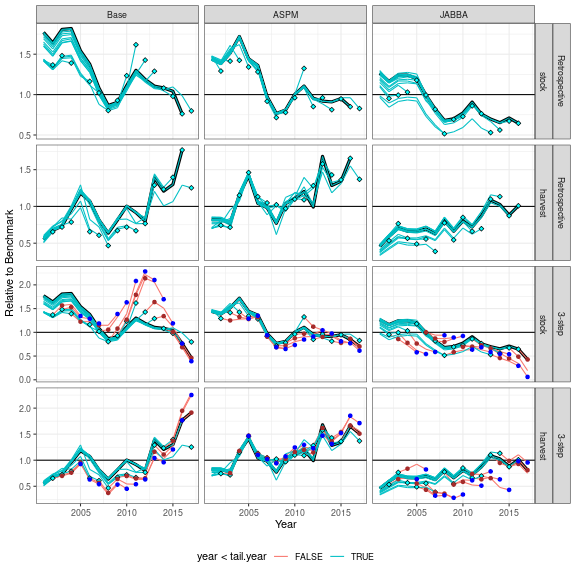
\includegraphics[width=6in]{figures/final-retro-all-1.png}
\caption{Retrospective analysis for the three models, points indicate the terminal years, and the think line the assessment using all the data.}
\label{fig:retro}
\end{figure*}

\begin{figure*}[htbp]
\centering
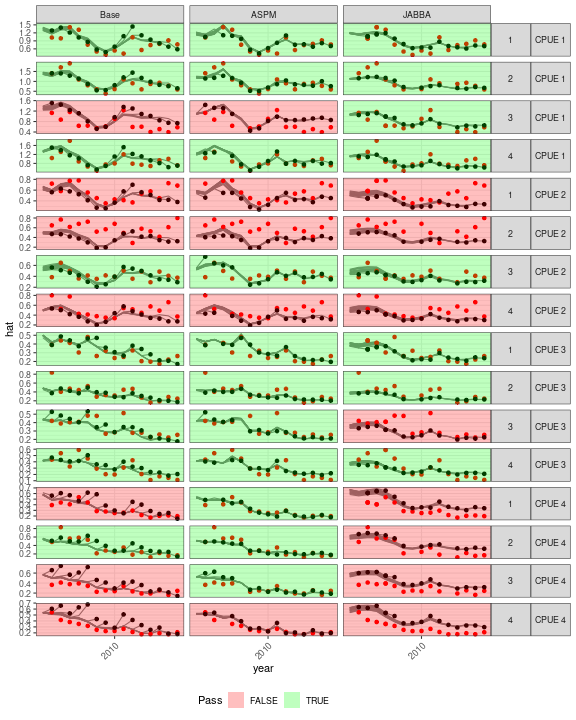
\includegraphics[width=6in]{figures/final-hy-plot-1.png}
\caption{Hindcasts for one step ahead predictions, red dots are the observed CPUE values and lines are the fits with terminal hincast year indicated by a point.}
\label{fig:hy}
\end{figure*}

\begin{figure*}[htbp]
\centering
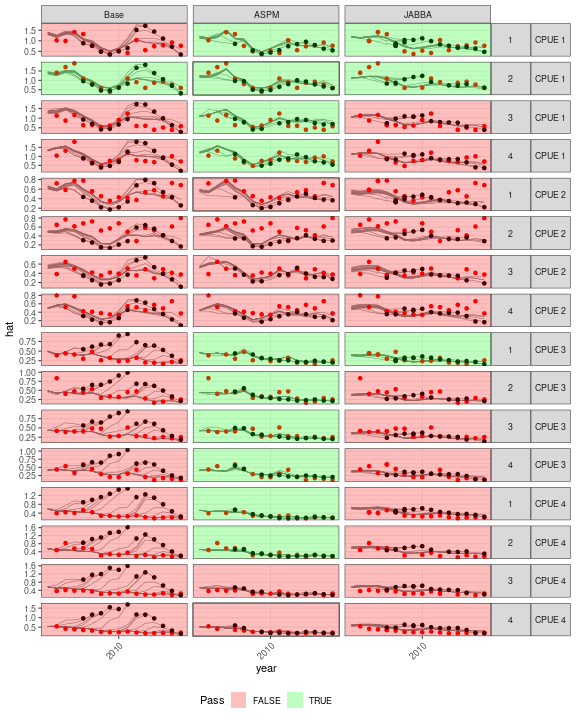
\includegraphics[width=6in]{figures/final-hy3-plot-1.png}
\caption{Hindcasts for three step ahead predictions, red dots are the observed CPUE values and lines are the fits with terminal hincast year indicated by a point.}
\label{fig:hy3}
\end{figure*}

\begin{figure*}[htbp]
\centering
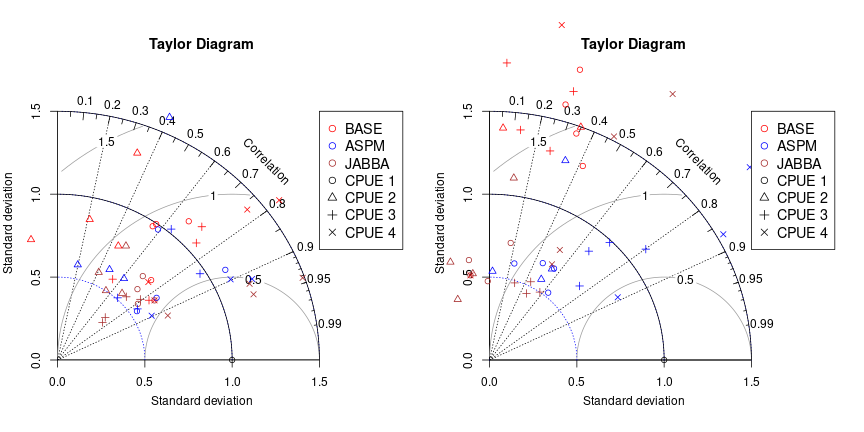
\includegraphics[width=6in]{figures/final-taylor-hy-1-1.png}
\caption{Taylor diagram for one and three year ahead predictions,  summarising the similarity between the observed time series of CPUEs and the predicted relative stock abundance. Each point quantifies how closely predictions match observations, the angle indicates the correlation, the centred root-mean-square error difference between the predicted and observed patterns is proportional to the distance to the point on the x and the contours around this point indicate the RMSE values; the standard deviations of the predictions are proportional to the radial distance from the origin, scaled so the observed pattern has a value of 1. The open circle corresponds to a series which is identical to the reference series. The colours correspond to the model and shape to the survey.)}
\label{fig:td}
\end{figure*}

\begin{figure*}[htbp]
\centering
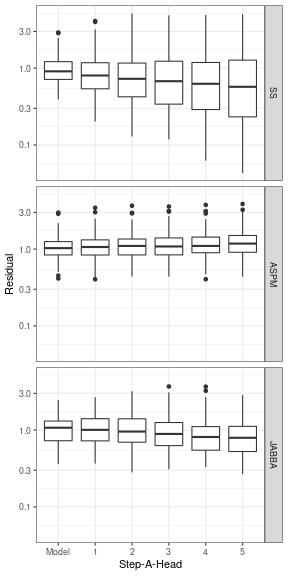
\includegraphics[width=4in]{figures/final-rsdl-1.png}
\caption{Residual for model (Step 0) and predictiion residuals for 1,2,3,4 and 5 steps ahead.}
\label{fig:residuals}
\end{figure*}

\clearpage
\newpage
\subsection{Appendix}
\label{metrics}

\appendix* 
\subsection{Metrics}

A well-fitting model results in predicted values close to the reference values, i.e. if $Y_t$ is the variable of interest at time $t$ and ${\hat{Y}_t}$ is it's predicted value then the prediction error is $e_t = Y_t - \hat{Y}_t$ and should be small. The accuracy of the predictions can be assessed by various measures. One example is the Mean Absolute Error (MAE), which is the mean of the absolute errors and measures how big of an error the forecast will generate on average.

\begin{equation} 
{MAE} =\frac{\sum_{i=1}^{n}\left|e_{i}\right|}{n}
\end{equation} 
 
A problem with the MAE is that the relative size of the error is not always obvious. Sometimes it is hard to tell a big error from a small error. To deal with this problem, the MAPE can be calculated instead, i.e. MAE as a percentage, this allows forecasts of different series in different scales to be compared.

\begin{equation} 
{MAPE = \frac{1}{T} \sum_{t=1}^T 100\, \left|\frac{e_t}{Y_t}\right|} 
\end{equation}

Both MAE and MAPE are based on the mean absolute error and so may understate the impact of big, but infrequent, errors.  To adjust for large rare errors the Root Mean Square Error (RMSE) squares the errors before calculating their mean i.e.
     
\begin{equation} 
{E^{\prime} = \sqrt{\frac{1}{T} \sum_{t=1}^T e_t^2}} 
(better to say RMSE like other measures for consistency?)
\end{equation}

This is the square root of the variance of the residuals (strictly if the mean of the residuals is 0 and practically if that is nearly 0) and indicates how close predicted values are close to the observations. As the square root of a variance it can also be interpreted as the standard deviation of the unexplained variance, and so lower values indicate better fits. Although RMSE,is commonly used when simulation testing assessment models \citep[e.g.][]{horbowy2011comparison} as described above it does not describe average error alone, is sensitive to outliers, favours forecasts that avoid large deviations from the mean, and cannot be used to compare across series.

The best statistical measure to use depends on the objectives of the analysis and using more than one measure can be helpful in providing insight into the nature of observation and process error structures. For example the correlation ($\rho$) between $Y_y$ and $\hat{Y_y}$ is not affected by the amplitude of the variations, is insensitive to biases and errors in variance, and can be used to compare across series.

$E^{\prime 2}$ and $\rho$ are related by the cosine rule i.e

\begin{equation} 
{E^{\prime 2} = \sigma_o^2 + \sigma_f^2 - 2\sigma_o\sigma_f\rho},
\end{equation}

where the reference set ($o$) are the observations ($Y_t$) not included in the retrospective assessment and the values (f) are their estimates ${\hat{Y}_t}$. This means that $E^\prime$, $\rho$ and $\sigma_f$ can be summarised simultaneously  \citep{taylor2001summarizing}. Taylor diagrams therefore provide a concise statistical summary of how well patterns match each other and are therefore especially useful for evaluating multiple aspects or in gauging the relative skill of different models \citep{griggs2002climate}. We can also compare RMSE and MAE to determine whether the forecast contains large but infrequent errors. The larger the difference between RMSE and MAE the more inconsistent the error size.

A more robust and easier to interpret statistic for evaluating prediction skill is the Mean Absolute Scaled Error (MASE) \citep{hyndman2006another}. MASE evaluates a model’s prediction skill relative to a na\ddot{i}ve baseline prediction. A prediction is said to have skill if it improves the model forecast compared to the baseline. A widely used baseline forecast for time series is the persistence algorithm that simply takes the value at the previous time step to predict the expected outcome at the next time step as a na\ddot{i}ve in-sample prediction, i.e. tomorrow will the same as today 

The MASE score scales the mean absolute error of the forecasts by the mean absolute error of a na\ddot{i}ve in-sample prediction, such that:

For a series of $T$ observations and predictions

\begin{equation} 
{MASE=\frac{\frac{1}{T} \sum_{t=1}^{T} \left|e_{t}\right|}
{\frac{1}{T-1} \sum_{t=2}^{T} \left|Y_{t+1}-Y_{t}\right|}}
\end{equation}

The MASE has the desirable properties of scale invariance, predictable behaviour, symmetry, interpretability and asymptotic normality. The scale invariance of MAPE and MASE allows us to compare forecasts across data sets with different scales, while MAE does not have such a feature. When it comes to the predictable behavior, percentage forecast accuracy measures rely on division of $y_{t}$, skewing the distribution of the MAPE for values of $y_{t}$ near or equal to 0. This is especially problematic for data sets whose scales do not have a meaningful 0, such as temperature in Celsius or Fahrenheit, and for intermittent demand data sets, where $y_{t}=0$  occurs frequently. With respect to symmetry, the MASE penalises positive and negative forecast errors equally, and penalises errors in large forecasts and small forecasts equally. The MASE can also be easily interpreted, as values greater than one indicate that in-sample one-step forecasts from the na\ddot{i}ve method perform better than the forecast values under consideration, in other words model forecasts are worse than a random walk. Conversely, a MASE score of 0.5 indicates that the model forecasts twice as accurate as a na\ddot{i}ve baseline prediction; thus the model has prediction skill.

[I now realized you used \iffalse.... I re-do...] 

\iffalse
If $Y_t$ is a variable of interest at time $t$ and \eqn{\hat{Y}_t} is it's predicted value then the prediction error is given by $e_t = Y_t - \hat{Y}_t$. For a series of $T$ observations and predictions The accuracy of the predictions can be compared to the actual value by calculating various measures, such as as the Mean Absolute Error (MAE), which is the mean of the absolute errors and tells us how big of an error we can expect from the forecast on average. \\

\eqn{MAE=\frac{\left|e_t\right|}{T}} \\

A problem with the MAE is that the relative size of the error is not always obvious. Sometimes it is hard to tell a big error from a small error. To deal with this problem, we can compute the MAPE instead, i.e. MAE as a percentage, this allows forecasts of different series in different scales to be compared.\\

\eqn{MAPE = \frac{1}{T} \sum_{t=1}^T 100\, \left|\frac{e_t}{Y_t}\right|}\\

Both MAE and MAPE are based on the mean error and so may understate the impact of big, but infrequent, errors. If we focus too much on the mean, we will be caught off guard by the infrequent big error. To adjust for large rare errors, we calculate the Root Mean Square Error (RMSE). By squaring the errors before we calculate their mean and then taking the square root of the mean, we arrive at a measure of the size of the error that gives more weight to the large but infrequent errors than the mean.\\

\eqn{RMSE = \sqrt{\frac{1}{T} \sum_{t=1}^T e_t^2}} \\

We can also compare RMSE and MAE to determine whether the forecast contains large but infrequent errors. The larger the difference between RMSE and MAE the more inconsistent the error size.
 
Another measure is the Mean Absolute Scaled Error (MASE) \\

\eqn{MASE={\frac {\sum _{t=1}^{T}\left|e_{t}\right|}{{\frac {T}{T-1}}\sum _{t=1}^{T}\left|Y_{t+1}-Y_{t}\right|}}} \\

Which has the desirable properties of scale invariance, predictable behaviour, symmetry, interpretability and asymptotic normality
 
The mean absolute scaled error is independent of the scale of the data, so can be used to compare forecasts across data sets with different scales. Behaviour is predictable as $y_{t}\rightarrow 0$] Percentage forecast accuracy measures such as the Mean absolute percentage error (MAPE) rely on division of $y_{t}$, skewing the distribution of the MAPE for values of $y_{t}$ near or equal to 0. This is especially problematic for data sets whose scales do not have a meaningful 0, such as temperature in Celsius or Fahrenheit, and for intermittent demand data sets, where $y_{t}=0$  occurs frequently.

Symmetry since The mean absolute scaled error penalises positive and negative forecast errors equally, and penalises errors in large forecasts and small forecasts equally. In contrast, the MAPE  fail both of these criteria. The mean absolute scaled error can be easily interpreted, as values greater than one indicate that in-sample one-step forecasts from the naïve method perform better than the forecast values under consideration.The Diebold-Mariano test for one-step forecasts is used to test the statistical significance of the difference between two sets of forecasts. To perform hypothesis testing with the Diebold-Mariano test statistic, it is desirable for $DM ∼ N ( 0 , 1 )$ $DM\sim N(0,1)$ , where $DM$ is the value of the test statistic. The DM statistic for the MASE has been empirically shown to approximate this distribution, while the mean relative absolute error (MRAE), MAPE and sMAPE do not.
 
Another measure is Theil's $U$\\
  
\eqn{U= \sqrt{\frac{1}{T}\\
     \sum_{t=1}^{T-1} \left(\frac{e_{t+1}}{Y_t}\right)^2
     \cdot \left[
    \frac{1}{T} \sum_{t=1}^{T-1} 
        \left(\frac{Y_{t+1} - Y_t}{Y_t}\right)^2 \right]^{-1}}}

The more accurate the forecasts, the lower the value of Theil's $U$,   which has a minimum of 0. This measure can be interpreted as the ratio of the RMSE of the proposed forecasting model to the RMSE of  a na\"ive model which simply predicts $Y_{t+1} = Y_t$ for all $t$. The na\"ive model yields $U = 1$; values less than 1 indicate an  improvement relative to this benchmark and values greater than 1 a deterioration.

Altough the methods have their limitations, they are simple tools for evaluating forecast accuracy that can be used without knowing anything about the forecast except the past values of a forecast.

Just because a forecast has been accurate in the past, however, does not mean it will be accurate in the future. Over fitting may make the forecast less accurate and there is always the possibility of an event occurring that the model cannot anticipate, a black swan event. When this happens, you don’t know how big the error will be. Errors associated with these events are not typical errors, which is what the statistics above try to measure. So, while forecast accuracy can tell us a lot about the past, remember these limitations when using forecasts to predict the future.

\fi


\end{document}

\section{Introduction}
\label{sec1}

It is assumed that the author is familiar with either plain
\TeX, \AmS-\TeX{} or a standard \LaTeX\ setup and, hence,
only the essential points are described in this document.
Nevertheless, we hope that this document is generally sufficient
for describing the requirements for preparation of
manuscripts. For more details, please see the \textit{\LaTeX{} User's Guide} or
\textit{The not so short introduction to \LaTeXe}.


\section{Installation}
\label{sec2}

Provided with \verb+ouparticle.cls+ are the files
\verb+sample.tex+ (this document explains the various
features of \verb+ouparticle.cls+) and \verb+sample.pdf+
(how the output using \verb+sample.tex+ should be). Your
paper can be compiled with standard \LaTeX,
preferably with the current \LaTeXe\ version. It will probably work
with older versions of \LaTeXe; however, this has not been
tested. The file \verb+ouparticle.cls+ needs to be copied
into a directory where \TeX\ looks for input files. The other files
need to be kept as a reference while preparing
your manuscript. Please use the predefined commands from \verb+sample.tex+ for title,
authors, abstract, body, etc.


\section{Preparing your manuscript}
\label{sec3}

\subsection{General guidelines}
\label{sec3.1}

\begin{enumerate}
\item
\LaTeX\ and \AmS-\LaTeX\ provide a rich set of commands for all common, important
features of your paper. Use them; avoid definitions and use of custom commands.

\item
There is no need to redefine any \TeX, \LaTeX\ or \AmS-\LaTeX\ commands.

\item
Avoid direct formatting for headings cleanly set as section headings.

\item
Use \LaTeX\ commands for font changes. For example: use \verb+\textbf{phrase}+,
not \verb+{\bf phrase}+; use \verb+\mathcal{C}+, not \verb+{\cal C}+; etc.
\end{enumerate}


\subsection{How to start with \texttt{ouparticle.cls}}
\label{sec3.2}

Before you type anything that actually appears in the paper, you need to
include a \verb+\documentclass{ouparticle}+ command at the very beginning,
and then the two commands that have to be part of any \LaTeX\ document,
\verb+\begin{document}+ at the start and \verb+\end{document}+ at the
end of your paper.


\subsection{Document structure}
\label{sec3.3}

The main structure of your paper is as follows:

\begin{verbatim}
\documentclass[12pt,...]{ouparticle}
\usepackage[...]{packages}

\title{...}
\author{
    \name{...}
    \address{...}
    \email{...}
        \and
    \name{...}
    \address{...}
    \email{...}
        \and
    \name{...}
    \address{...}
    \email{...}
}
\abstract{...}
\keywords{...}

\maketitle

\begin{document}

\section{....}
...
\subsection{....}
....
\end{document}
\end{verbatim}


\subsection{Options}
\label{sec3.4}

By default, all of the options within \verb+article.cls+ are available
with this class file. This class file provides the following additional options.

\begin{description}
\item \textbf{oneline:}
This option will set your entire manuscript in one line spacing.
It will not affect the footnote, figure and table environments.

\item \textbf{halfline:}
This is to set your entire manuscript in half line spacing.

\item \textbf{endnotes:}
To make all footnotes to endnotes. You may follow the same
coding \verb+\footnote{text}+ for both footnotes and endnotes. Once you use this option
you have to use the \verb+\theendnotes+ command at the place where all the endnotes
have to be set in your paper.

\item \textbf{numbib:}
This is the default option that numbers the bibliography items;
this option does nothing with natbib and other packages.

\item \textbf{nonumbib:} For unnumbered bibliography.
\end{description}


\subsection{Front matter}
\label{sec3.5}

The title of the manuscript is simply specified by using the \verb+\title{text}+ command in
the same manner as in this sample. Author's information consists of the name of the author
and the corresponding institutions with addresses, as given in this example. Include an
electronic mail address if available, inserting it into the \verb+\email{text}+ commands.
You may follow the same coding if there are more than one author; separate authors with
\verb+\and+. Please identify the corresponding author with his/her electronic
mail address by \verb+\thanks{text}+. An abstract for your paper is specified by using
\verb+\abstract{text}+. A \verb+\keywords{text}+ macro may also be used to indicate keywords for the
article. Use \verb+\maketitle+ after the abstract and keywords to make the header of your article.

\subsection{Sections and subsections}
\label{sec3.6}

To begin a new section, give the heading of that section in the \verb+\section{text}+ command.
A section number is supplied automatically. Use the starred form (\verb+\section*{text}+) of the
command to suppress the automatic numbering. If you want to be able to make reference to that section,
then you need to \texttt{label} it (see Section \ref{sec3.14}). You can have sections up to
five levels. The sectioning commands are \verb|\section|, \verb|\subsection|, \verb|\subsubsection|,
\verb|\paragraph| and \verb|\subparagraph|.

\subsection{Ordinary text}
\label{sec3.7}

The ends of words and sentences are marked by spaces. It does not matter how many
spaces you type. The end of a line counts as a space. One
or more blank lines denote the end of a paragraph.

There are a number of things for which you need to follow different
methods. As you know, quotation marks, quotes within quotes,
dashes, ellipsis, etc. should be as per the \LaTeX\ standard input. \LaTeX\ interprets some
common characters as commands, and therefore you must instead type those common characters as
specific \LaTeX\ commands to generate them. Those characters are \$, \&, \%, \#, \{, and \}.

\subsection{Formatting}
\label{sec3.8}

One should always use \LaTeX\ macros rather than the lower-level
\TeX\ macros like \verb+\it+, \verb+\bf+ and \verb+\tt+. The
\LaTeX\ macros offer much improved features. The following table summarizes the font
selection commands in \LaTeX.


\subsubsection*{\LaTeX\ text formatting commands}
\begin{tabular}{ll@{\hskip60pt}ll}
\verb+\textit+  & Italics      &\verb+\textsf+  & Sans Serif\\
\verb+\textbf+  & Boldface     &\verb+\textsc+  & Small Caps\\
\verb+\texttt+  & Typewriter   &\verb+\textmd+  & Medium Series\\
\verb+\textrm+  & Roman        &\verb+\textnormal+ & Normal Series\\
\verb+\textsl+  & Slanted      &\verb+\textup+  & Upright Series
\end{tabular}


\subsubsection*{\LaTeX\ math formatting commands}
\begin{tabular}{ll@{\qquad}ll}
\verb+\mathit+     & Math Italics            &\verb+\mathfrak+   & Fraktur\\
\verb+\mathbf+     & Math Boldface       &\verb+\mathbb+     & Blackboard Bold\\
\verb+\mathtt+     & Math Typewriter     &\verb+\mathnormal+ & Math Normal\\
\verb+\mathsf+     & Math Sans Serif     &\verb+\boldsymbol+ & Bold math for Greek letters\\
\verb+\mathcal+    & Calligraphic        &                   & and other symbols
\end{tabular}


\subsection{Figures and tables}
\label{sec3.9}

Use normal \LaTeX\ coding for figures and tables.
Figure and table environments should be inserted after (not in) the paragraph in which
the figure is first mentioned or grouped all
together at the end of the file. They will be numbered automatically.
The following is an example of typesetting a table.

\begin{verbatim}
\begin{table}
\caption{Table caption text.}
\label{key}
The table matter goes here.
\end{table}
\end{verbatim}

As always with \LaTeX, the \verb+\label+ must be after the
\verb+\caption+, and inside the figure or table environment. The reference for
figures and tables inside text can be made using the \verb|\ref{key}| command.


\subsection{Equations}\label{sec3.10}

Equations are used in the same way as described in the \LaTeX\ manual.
Do not start a paragraph with a displayed equation. Equations are numbered consecutively, with equation numbers
in parentheses flush right.
 For example, if you type
\begin{verbatim}
\begin{equation}\label{eq1}
\int^{r_2}_0 F(r,\varphi){\rm d}r\,{\rm d}\varphi = [\sigma r_2/(2\mu_0)]
\int^{\infty}_0\exp(-\lambda|z_j-z_i|)\lambda^{-1}J_1 (\lambda r_2)J_0
(\lambda r_i\,\lambda {\rm d}\lambda)
\end{equation}
\end{verbatim}
then you will get the following output:
\begin{equation}\label{eq1}
\int^{r_2}_0 F(r,\varphi){\rm d}r\,{\rm d}\varphi = [\sigma r_2/(2\mu_0)]\int^{\infty}_0
\exp(-\lambda|z_j-z_i|)\lambda^{-1}J_1 (\lambda r_2)J_0 (\lambda r_i\,\lambda {\rm d}\lambda)
\end{equation}
It inserts space both above and below the equation. \AmS-\LaTeX{} has several environments that
make it easier to typeset complicated multiline displayed equations. These are explained in the
\AmS-\LaTeX{} User Guide. A \verb+subequation+ environment is available to create equations with
sub-numbering of the equation counter. It takes one (optional)
argument to specify the way that the sub-counter should appear.


\subsection{Displayed text}
\label{sec3.11}

Text is displayed by indenting it from the left and right margins.
Quotations are commonly displayed. There are short
quotations:
\begin{quote}
   This is a short quotation.  It consists of a
   single paragraph of text.  See how it is formatted.
\end{quote}
and longer ones:
\begin{quotation}
   This is a longer quotation.  It consists of two
   paragraphs of text, neither of which are
   particularly interesting.

   This is the second paragraph of the quotation.  It
   is just as dull as the first paragraph.
\end{quotation}
You can even display poetry.
\begin{verse}
   There is an environment
    for verse \\             % The \\ command separates lines
   Whose features some poets % within a stanza.
   will curse.

                             % One or more blank lines separate stanzas.

   For instead of making\\
   Them do \emph{all} line breaking, \\
   It allows them to put too many words on a line when they'd rather be
   forced to be terse.
\end{verse}


\subsection{Listings}
\label{sec3.12}

Another frequently displayed structure is a list. The
following is an example of an \emph{itemized} list.
\begin{itemize}
   \item This is the first item of an itemized list.
         Each item in the list is marked with a
         `$\bullet$'.

   \item This is the second item of the list. It
         contains another list nested inside it. The
         inner list is an \emph{enumerated} list.
         \begin{enumerate}
            \item This is the first item of an enumerated
                  list that is nested within the
                  itemized list.

            \item This is the second item of the inner list.
                  \LaTeX\ allows you to nest lists
                  deeper than you really should.
         \end{enumerate}
         This is the rest of the second item of the
         outer list. It is no more interesting than
         any other part of the item.
   \item This is the third item of the list.
\end{itemize}


\subsection{Displayed sentences: theorems and such}
\label{sec3.13}

These environments have to be defined with the help of \LaTeX's \verb+\newtheorem+ command, and
also with the \AmS-\LaTeX\ package for theorems that is already with your class file.
For example, \verb+\newtheorem{thm}{Theorem}+. Predefined theorem styles can be used in your article
to differentiate the theorem-like environments. You can have an extra command, \verb+\newproof+,
that can be used for displayed text. The following is an example of using the above-defined
\verb+thm+ environment.
\begin{verbatim}
\begin{thm}
This is body matter for this environment.
\end{thm}
\end{verbatim}

\subsection{Cross-referencing}
\label{sec3.14}

\LaTeX\ possesses features for labelling and cross-referencing
section headings, equations, tables, figures and theorems.
Their proper usage in the context of section headings, equations,
tables and figures are discussed in the appropriate sections.

Cross-referencing depends upon the use of `keys' that are defined by the user.
The \verb+\label{key}+ command is used to identify the links. Keys are strings of
characters that serve to label section headings, equations, tables and figures
that replace explicit, by-hand numbering. The \verb+\ref{key}+ command is used for
cross-referencing.

Files that use cross-referencing (and almost all manuscripts do)
need to be processed through \LaTeX\ at least twice to
ensure that the keys have been properly linked to the appropriate numbers.

\subsection{Footnotes and endnotes}
\label{sec3.15}

The footnote text can either appear at the bottom of a page or at the end of your paper.
The \verb+\footnote+ macro \emph{should not} be used in the front matter to provide additional
information about authors (such as corresponding addresses); instead, use \verb+\thanks{text}+ commands.
The document option `\texttt{endnotes}' is used to make endnotes. The command \verb+\theendnotes+ should
be used to place the endnotes at the required location in the text. They will be put in a separate
`Notes' section.


\subsection{Appendix}
\label{sec3.16}

The \verb+\appendix+ command signals that all following sections are
appendices, and therefore the headings after \verb+\appendix+ will be set
as appendix headings. For a single appendix, use \verb+\appendix*+ followed by the \verb+\section{text}+
command to suppress the appendix letter in the section heading.


\subsection{Special sections for notes and acknowledgements}
\label{sec3.17}

If you wish to include a `Notes' or `Acknowledgements' section in your paper,
use the \verb+\begin{notes}...\end{notes}+ macro. We use the same environment for both
`Notes' and `Acknowledgements'. The following examples show to how to use this macro.
\begin{verbatim}
\begin{notes}
Please note that this class file is provided as it is, and
copyright by Oxford University Press. You are free to use this
class file, provided that you do not make changes in this class file.
If you do make changes, you are requested to rename the class file.
\end{notes}

\begin{notes}[Acknowledgements]
The authors would like to thank...
\end{notes}

\end{verbatim}


\subsection{References}
\label{sec3.18}

The reference entries can be \LaTeX\ typed bibliographies or generated through a BIB\TeX\ database.
BIB\TeX\ is an adjunct to \LaTeX\ that aids in the preparation of bibliographies. BIB\TeX\
allows authors to build up a database or collection of bibliography entries that may be used for many
manuscripts. They also save us the trouble of having to specify formatting. More details can be found
in the \textit{BIB\TeX\ Guide}. For \LaTeX\ reference entries use the
\verb+\begin{thebibliography}....\end{thebibliography}+ environment (see below) to make references in your paper.
We have provided the class file option to distinguish two styles of references. Those options are \verb+numbib+ and \verb+nonumbib+.
You can select one of these options with the \verb+\documentclass+ command. By default the class file will take the
\verb+numbib+ option. The following is an example of \LaTeX\ bibliography.

\begin{verbatim}
\begin{thebibliography}{0}
\bibitem{bib1}
Goossens, M., F. Mittelbach, and A. Samarin: {\em The {\LaTeX} Companion}.
Addison-Wesley, Reading, MA, USA, 1994.
\bibitem{bib2}
Knuth, D.E: {\em The {\TeX}book}. Addison-Wesley, Reading, MA, USA, 1984.
\bibitem{bib3}
Lamport, L.: {\em {\LaTeX} -- A Document Preparation System -- User's
Guide and Reference Manual}. Addison-Wesley, Reading, MA, USA, 1985.
\bibitem{bib4}
Smith, I.N., R.S. Johnes, and W.P. Hines: 1992, `Title of the Article',
\textit{Journal Title in Italics} \textbf{Vol. no. X}, pp. 00--00
\end{thebibliography}
\end{verbatim}


\section{Macro packages}
\label{sec4}

The following packages are compulsorily needed by the class file:
\begin{verbatim}
amsmath         graphicx
amssymb         endnotes
amsfonts        setspace
verbatim        geometry
\end{verbatim}

The commonly used packages already used by this class file that authors can use whenever required are:
\begin{verbatim}
xspace          latexsym        url
amscd           multicol        algorithm
rotating        array           subfigure
\end{verbatim}

Additionally, you can use other packages and these should be loaded
using the \verb+\usepackage+ command.

\end{document}
